\documentclass[12pt]{ucsd}
% documentclass options: default is 11pt, oneside, final.
% fonts: 10pt, 11pt, 12pt -- are valid for UCSD dissertations.
% sides: oneside, twoside -- note that two-sided theses are not accepted by OGS
% mode: draft, final -- draft mode switches to single spacing, removes hyperlinks,
%                       and places a black box at every overfull hbox (check these before submission).
% chapterheads -- include this if you want your chapters to read:
% Chapter 1
% Title of Chapter
%
% instead of
%
% 1 Title of Chapter

% Input and configure the required packages.
% UCSD Mathematics Dissertation Template
%
% Please read the comments in this file and make appropriate edits.
% NOTE: Always refer to the ``Preperation and Submission Manual for
% Doctoral Dissertations and Masters Theses for 20**'', where 20** is
% the year of your graduation, for officiation preparations guidelines.
%
% If you desire more control, please see the attached files:
%   * ucsd.cls -- Class file
%   * uct10.clo, uct11.clo, uct12.clo -- Configuration files for font sizes 10pt,11pt,12pt
%
% CHANGELOG:
%   * Original file adapted from brockman.tex by JRB and RMR
%     to work with ucsd.cls

% Include all packages you need here.  Some standard options are suggested below.

% GEOMETRY - This will force the use of Letter paper.
% Many TeX installations default to A4 paper.  The formatting
% of the thesis class file requires Letter, else the margins
% will be wrong when you go to print it (and OGS will complain).
% If your TeX implementation is not setup for Letter paper, and
% you cannot change it, uncommenting the following line may fix
% problem.
% \usepackage[paper=letterpaper]{geometry}


%% AMS PACKAGES - Chances are you will want some or all of these if writing a math dissertation.
% \usepackage{amsmath, amscd, amssymb, amsthm}

%% GRAPHICX - This is the standard package for including graphics for latex/pdflatex.
% \usepackage{graphicx}

%% LATIN MODERN FONTS (replacements for Computer Modern)
% \usepackage{lmodern}
% \usepackage[T1]{fontenc}

%% INDEX
% Uncomment the following two lines to create an index:
% \usepackage{makeidx}
% \makeindex
% You will need to uncomment the \printindex line near the
% bibliography to display the index.  Use the command
% \index{keyword} within the text to create an entry in the index
% for keyword.

%% HYPERLINKS
% To create a PDF with hyperlinks, you need to include the hyperref package.
% THIS HAS TO BE THE LAST PACKAGE INCLUDED!
% Note that the options plainpages=false and pdfpagelabels exist
% to fix indexing associated with having both (ii) and (2) as pages.
% Also, all links must be black according to OGS.
% See: http://www.tex.ac.uk/cgi-bin/texfaq2html?label=hyperdupdest
% Note: This may not work correctly with all DVI viewers (i.e. Yap breaks).
% NOTE: hyperref will NOT work in draft mode, as noted above.
% \usepackage[colorlinks=true, pdfstartview=FitV, linkcolor=black, citecolor=black, urlcolor=black,plainpages=false,pdfpagelabels]{hyperref}
% \hypersetup{ pdfauthor = {Your Name Here}, pdftitle = {The Title of The Dissertation}, pdfkeywords = {Keywords for Searching}, pdfcreator = {pdfLaTeX with hyperref package}, pdfproducer = {pdfLaTeX}}

\usepackage{amsmath,amsfonts,amsthm,amssymb}
\usepackage{setspace}
\usepackage{fancyhdr}
\usepackage{lastpage}
\usepackage{extramarks}
\usepackage{chngpage}
\usepackage{soul}
\usepackage[usenames,dvipsnames]{color}
\usepackage{graphicx,float,wrapfig}
\usepackage{ifthen}
\usepackage{listings}
\usepackage{courier}
\usepackage[bw,framed,numbered]{mcode}
\usepackage{microtype}
\usepackage{appendix}
\usepackage{hyperref}
\usepackage[all]{hypcap}
\usepackage{url}

% Needed for changing the font size in \documentclass{} while
% using the fancyhdr package. Else the warning:
% \headheight is too small (12.0pt):Make it at least 14.49998pt.
\setlength{\headheight}{15pt}

% For faster processing, load Matlab syntax for listings
\definecolor{MyDarkGreen}{rgb}{0.0,0.4,0.0}
\lstloadlanguages{Matlab}%
\lstset{language=Matlab,
       frame=single,
       basicstyle=\scriptsize\ttfamily,
       keywordstyle=[1]\color{Blue}\bf,
       keywordstyle=[2]\color{Purple},
       keywordstyle=[3]\color{Blue}\underbar,
       identifierstyle=,
       commentstyle=\usefont{T1}{pcr}{m}{sl}\color{MyDarkGreen}\small,
       stringstyle=\color{Purple},
       showstringspaces=false,
       tabsize=5,
       % Put standard MATLAB functions not included in the default
       % language here
       morekeywords={xlim,ylim,var,alpha,factorial,poissrnd,normpdf,normcdf},
       % Put MATLAB function parameters here
       morekeywords=[2]{on, off, interp},
       % Put user defined functions here
       morekeywords=[3]{FindESS},
       morecomment=[l][\color{Blue}]{...},
       numbers=left,
       firstnumber=1,
       numberstyle=\tiny\color{Blue},
       stepnumber=0
       }

% Adds a hyperlink to an email address.
\newcommand{\mailto}[2]{\href{mailto:#1}{#2}}

% Homework Specific Information
\newcommand{\thesisTitle}{Master's Thesis}
\newcommand{\thesisSubTitle}{Robot Traffic School}
\newcommand{\thesisAuthorName}{Thomas Denewiler}
\newcommand{\thesisAuthorEmail}{tdenewiler@gmail.com}

% These commands set the document properties for the PDF output. Needs the hyperref package.
\hypersetup
{
    colorlinks,
    linkcolor={black},
    citecolor={black},
    filecolor={black},
    urlcolor={black},
    pdfauthor={\thesisAuthorName <\mailto{\thesisAuthorEmail}{\thesisAuthorEmail}>},
    pdfsubject={\thesisTitle},
    pdftitle={\thesisTitle},
    pdfkeywords={UC San Diego, Small Unmanned Ground Vehicles, Robotics},
    pdfstartpage={1},
}

% Includes a MATLAB script.
% The first parameter is the label, which also is the name of the script.
% The second parameter is the optional caption.
\newcommand{\matlabscript}[2]
  {\begin{itemize}\item[]\lstinputlisting[caption=#2,label=#1]{#1}\end{itemize}}

% User defined macros.
\def\argmin{\mathop{\arg\,\min}\limits}
\def\argmax{\mathop{\arg\,\max}\limits}
\def\argsol{\mathop{\arg\,\text{sol}}\limits}


% Uncomment this line to compile a subset of the chapters.
% \includeonly{chapters/chIntroduction}

% Document starts here.
\begin{document}

% Document specific information.
%% REQUIRED FIELDS -- Replace with the values appropriate to you
\title{Robot Traffic School}
% No symbols, formulas, superscripts, or Greek letters are allowed
% in your title.

\author{Thomas Denewiler}
\degreeyear{2010}
\degree{Master's of Science}
% Master's Degree theses will NOT be formatted properly with this
% file.

\field{Mechanical and Aerospace Engineering}
\chair{Professor Thomas Bewley}
% Uncomment the next line iff you have a Co-Chair
% \cochair{Professor Cochair Semimaster}
% \othermembers{%  These must be alpha by last name.
% Professor Humor Less\\
% Professor Ironic Name\\
% Professor Cirius Thinker\\
% }
\numberofmembers{1} % |chair| + |cochair| + |othermembers|


% The title, copyright, and signature pages.
\begin{frontmatter}
\makefrontmatter
% No symbols, formulas, superscripts, or Greek letters are allowed
% in your title.
\title{Robot Traffic School}
\author{Thomas Denewiler}
\degreeyear{2010}
\degree{Master of Science}
\field{Mechanical and Aerospace Engineering}
\chair{Professor Thomas R. Bewley}

% Uncomment the next line iff you have a Co-Chair
% \cochair{Professor Cochair Semimaster} 
%
% Or, uncomment the next line iff you have two equal Co-Chairs.
%\cochairs{Professor Chair Masterish}{Professor Chair Masterish}

%  The rest of the committee members  must be alphabetized by last name.
\othermembers{
Professor 2 \\ 
Professor 3 \\
}
\numberofmembers{3} % |chair| + |cochair| + |othermembers|

%% START THE FRONTMATTER
\makeatletter
\let\@currsize\normalsize
\begin{frontmatter}
\makefrontmatter

%% DEDICATION
% You have three choices here:
%   1. Use the ``dedication'' environment.   Put in the text you want,
%   and you'll get a perfectly respectable dedication page.
%
%   2. Use the ``mydedication'' environment.  If you don't like the
%   formatting of option 1, use this environment and format things
%   however you wish.
%
%   3. If you don't want a dedication, it's not required.
\begin{dedication} % The style file will format this for you.
To Grandma Denny, \\
it's a small step from board games to Kalman filters, \\
To my parents, \\
for their time and encouragement in everything.
\end{dedication}

% \begin{mydedication} % You are responsible for formatting here.
%   \vspace{1in}
%   \begin{flushleft}
% 	To me.
%   \end{flushleft}
%
%   \vspace{2in}
%   \begin{center}
% 	And you.
%   \end{center}
%
%   \vspace{2in}
%   \begin{flushright}
% 	Which equals us.
%   \end{flushright}
% \end{mydedication}


%% EPIGRAPH
%  The same choices that applied to the dedication apply here.

% \begin{epigraph} % The style file will position the text for you.
%   \emph{A careful quotation\\
%   conveys brilliance.}\\
%   ---Smarty Pants
% \end{epigraph}

% \begin{myepigraph} % You position the text yourself.
%   \vfil
%   \begin{center}
%     {\bf Think! It ain't illegal yet.}
%
% 	\emph{---George Clinton}
%   \end{center}
% \end{myepigraph}

\tableofcontents
\listoffigures  % Uncomment if you have any figures
\listoftables   % Uncomment if you have any tables


%% ACKNOWLEDGEMENTS
%  While technically optional, you probably have someone to thank.
%  Also, a paragraph acknowledging all coauthors and publishers (if
%  you have any) is required in the acknowledgements page and as the
%  last paragraph of text at the end of each respective chapter. See
%  the OGS Formatting Manual for more information.

\begin{acknowledgements}
The enthusiasm and energy of Professor Thomas Bewley has been an inspiration and his support and advice have been invaluable.

I am grateful to Gideon Prior, Nima Ghods, Amin Rahimi and Steve Stancliff for our many long conversations while learning how to build better robots.

I would also like to thank Mike Bruch and the ACS team (Gaurav Ahuja, Donnie Fellars, Greg Kogut and Brandon Sights) at SPAWAR for their support.

And without the love and encouragement from Silvie I would not have made it this far.
\end{acknowledgements}


%% VITA
%  A brief vita is required in a doctoral thesis. See the OGS
%  Formatting Manual for more information.
% \begin{vitapage}
% \begin{vita}
%   \item[2002] B.~S. in Mathematics \emph{cum laude}, University of Southern North Dakota, Hoople
%   \item[2002-2007] Graduate Teaching Assistant, University of California, San Diego
%   \item[2007] Ph.~D. in Mathematics, University of California, San Diego
% \end{vita}
% \begin{publications}
%   \item Your Name, ``A Simple Proof Of The Riemann Hypothesis'', \emph{Annals of Math}, 314, 2007.
%   \item Your Name, Euclid, ``There Are Lots Of Prime Numbers'', \emph{Journal of Primes}, 1, 300
% 	B.C.
% \end{publications}
% \end{vitapage}

%% Abstract
% Doctoral dissertation abstracts should not exceed 350 words. MS thesis
% abstracts can be up to 250 words. The abstract may, however, continue to a
% second page if necessary.
\begin{abstract}
Increasing the autonomous performance of robots increases the complexity of possible behaviors that can be implemented and their utility to end users. To that end the state estimation and control algorithms for EOD differential drive robots have been studied and improved by incorporating a low-cost compass and encoders to the sensor suite, generating better noise models for the extended Kalman filter and implementing a nonlinear model-based controller. A DGPS system was built and temporarily integrated with the standard robot sensors to measure ground truth positions which were used to find more accurate system and measurement noise covariance values for use with the Kalman filter. Independently a control Lyapunov function was found based on differential drive robot kinematics to output a suitable control law and the results are compared with the previously existing PID controller, especially in regards to the benefits of asymptotic stability. The improved robot performance was implemented using robots and an OCU that are currently fielded and will accelerate development of advanced maneuvers such as retrotraverse over long distances.
\end{abstract}

\end{frontmatter}
\makeatother

\end{frontmatter}

% Meat and potatoes.
\chapter{Introduction}
\label{ch:introduction}
In this chapter we give a brief overview of autonomous navigation and the small unmanned ground vehicles (UGVs) that will be considered in this thesis. We also describe some of the issues in state estimation and controls that were considered during research in improving the autonomous driving behaviors of the UGVs.

\section{The Need for Autonomy}
\label{sec:needforautonomy}
Robots have been developed to assist humans in tasks that are generally considered dirty, dangerous or boring. Recently robots have found a useful niche as a tool to help Expolosives Ordinance Disposal (EOD) teams to assess and eliminate threats due to improvised explosive devices (IEDs), commonly referred to as roadside bombs, by allowing humans to maintain a safe stand-off distance while investigating a scene. Clearly this falls under the dangerous category. The current method that EOD teams use involves teleoperation of the robot to get from the base to the object of interest. In the process of teleoperating the robot the operator is exposed and vulnerable to other external threats in the area. As technologies mature to provide humans with better tools shortcomings are discovered, such as the vulnerability due to teleoperation, and that opens up avenues for improvement in the development of these tools. For robots one approach to reducing the amount of work humans are required to perform is to give the robots more intelligence via autonomous behaviors using additional sensors, more specialized actuators and software to automate the largest amount of routine tasks as possible.

When adding autonomy to robots nearly all of the tasks can be summarized by the following questions:
\begin{itemize}
\item Where am I?
\item What's around me?
\item Where do I want to go?
\item How do I get there?
\end{itemize}

Other tasks for small UGVs include sending them into buildings that are dangerous due to structural damage or unknown, possibly hostile elements inside so that the robots can map the interior and additionally to provide human operators with images to assess the danger prior to any humans entering the buildings \cite{CongressUGV06}. After the attacks on the World Trade Center on September 11, 2001 several small UGV systems were used to look for survivors in the rubble and to help assess structural damage to nearby buildings \cite{Everett02}.

The initial attempt at adding autonomy to the EOD robots resulted in somewhat erratic driving behavior, especially near obstacles, as the robot trajectory would not be smooth as it changed speed and attempted to make small corrections to its original path to move around the obstacle. In this thesis we will look at smoothing out the trajectories taken by the robot by looking for improvements in the state estimation (Where am I?) and controls (How do I get there?) algorithms. This work ignores actual obstacle detection (What's around me?) and will be using a simple planning algorithm (Where do I want to go?) to simulate obstacles in the robot path which will force the robot to change direction and speed multiple times.

*** Talk about how speed and efficiency are important characteristics of robots in their typical operating environments and that improved navigation would improve the speed and efficiency. An example is less time waiting to get robot close to IED or to clear a building means less time for humans in hostile environment. In search and rescue situations this would lead to less time for searching and more time for rescuing. With improved autonomy more advanced behaviors, such as retrotraverse, become possible to implement. ***

\section{Thesis Outline \& Contributions}
\label{sec:outline}
The problem of autonomous navigation is not isolated to any one technical area but is instead a combination of sensor integration to allow the robot position and obstacles to be observable, noise filtering, state estimation and control algorithms. As much as possible this research has attempted to isolate the effects of each of those areas to enable a quantitative analysis to determine which parts of the system contribute the largest effect on overall robot behavior.

Chapter \ref{ch:background} gives some background on the types of robots used, the sensors on the robots and the operator control unit (OCU). Chapter \ref{ch:estimation} presents the state estimation algorithm that is used on the robots. Chapter \ref{ch:controls} discusses the original control algorithm and a new control algorithm applied as part of this research. Chapter \ref{ch:results} gives the results of experiments run with the robots and looks at the main contributing factors for smooth autonomous navigation. Chapter \ref{ch:futurework} suggests future avenues of research to pursue. The conclusion is found in Chapter \ref{ch:conclusion}.

The main contribution of this research is that the small UGVs investigated here have greater autonomy which will allow for less human oversight of basic functionality. This is especially important for the dirty, dangerous and boring tasks where robots are most useful because it allows humans to focus their concentration, time and effort on being clean, safe and efficient.
\chapter{Background}
\label{ch:background}
*** Put in a description of the PackBot, Talon and Urbot along with a description of the algorithms originally used and the results obtained using those algorithms. Talk about JAUS and MOCU a little bit. Discuss more about how the robots are used by EOD. Include that for robots to drive around on their own all they require is an estimate of where they are, a path to follow, a controller to determine the actuator outputs and motor controllers to perform the controller outputs. ***

*** It might be best to have more of a description of the actual problem here along with a description of the testing area. ***

\section{Small Unmanned Ground Vehicles}
\label{sec:smallugvs}
The PackBot is manufactured by iRobot. *** Add more. ***

The Talon is manufactured by Foster Miller. *** Add more. ***

The Urbot is an experimental prototype of a small UGV developed by SSC-SD and is shown in Figure \ref{fig:urbot}. *** Add more. ***

*** Say that each of the robots has a standard sensor suite and list what those sensors are. ***

\begin{figure}[ht!]
	\centering
	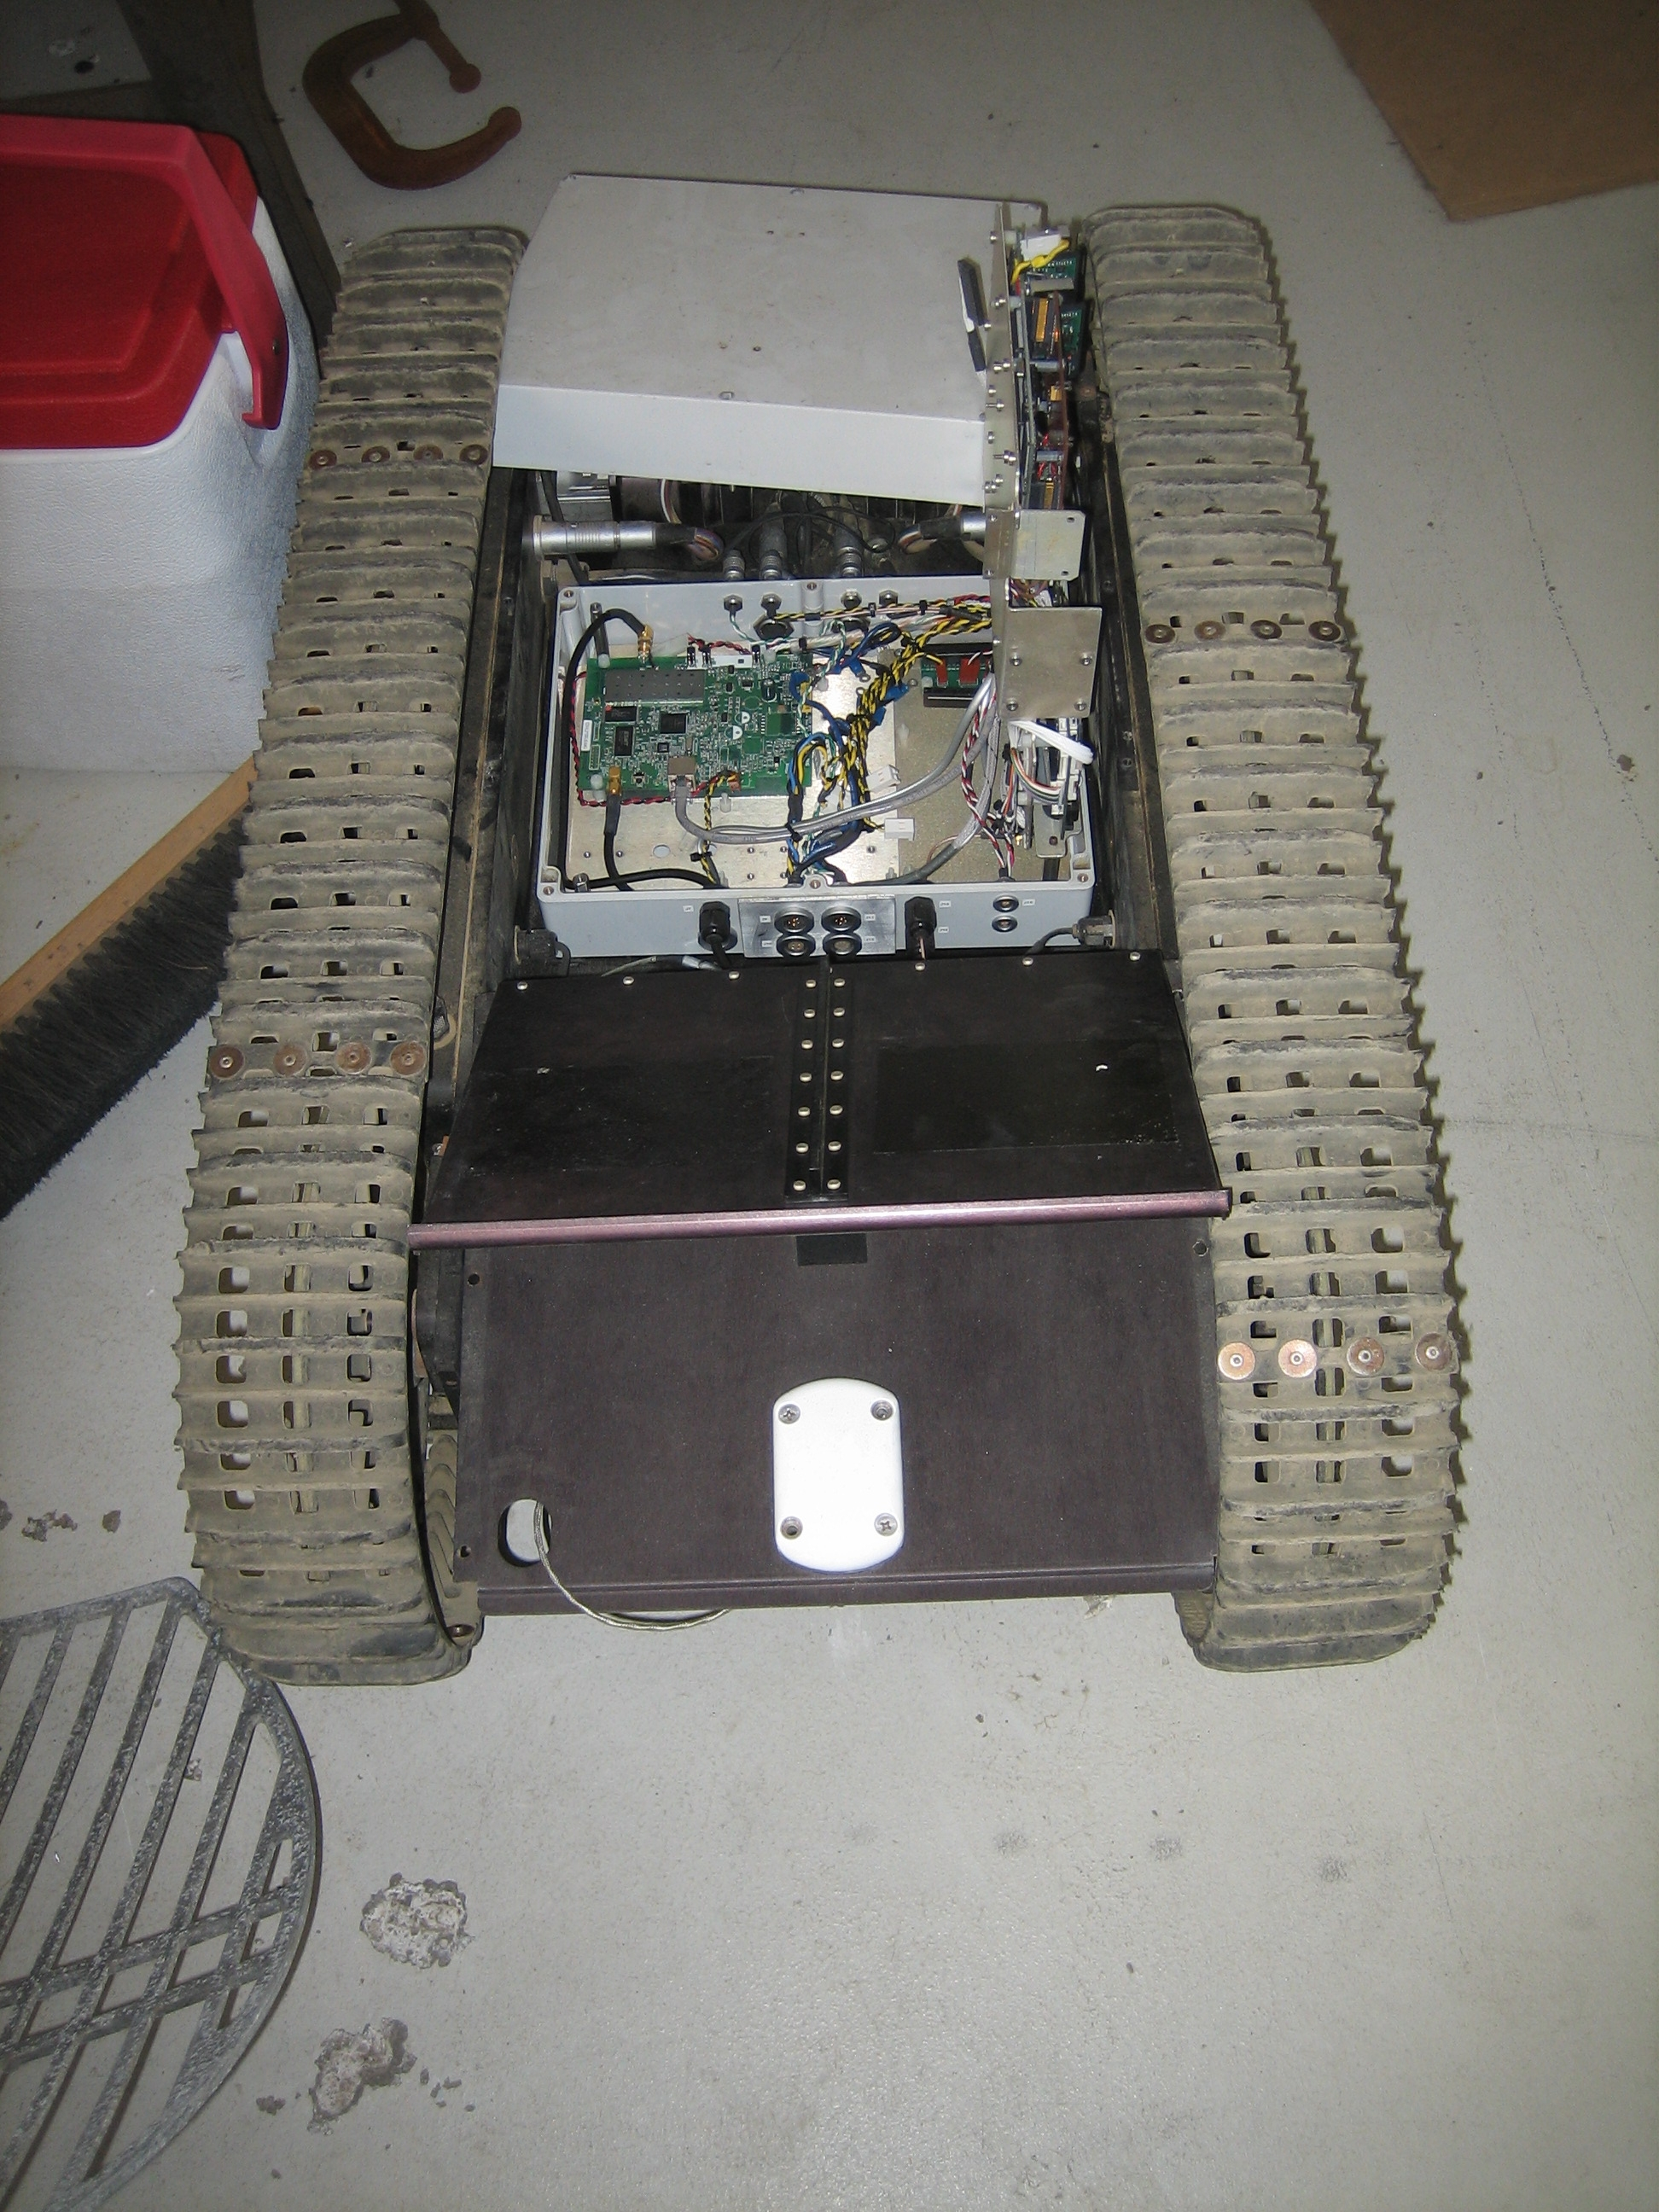
\includegraphics[width=.5\textwidth]{images/urbot}
	\caption{Urbot.}
	\label{fig:urbot}
\end{figure}

\section{MOCU \& JAUS}
\label{sec:mocujaus}
The Multi-Robot Operator Control Unit (MOCU) is a highly configurable front-end for simultaneous command and control of multiple systems and was created at SSC-SD \cite{PowellMOCU08}. MOCU has the ability to use a variety of communications protocols for interfacing to different systems and uses the Joint Architecture for Unmanned Systems (JAUS) to send and receive data to all of the UGVs used in this research \cite{RoweJAUS08}.

\section{The Duals: Estimation \& Controls}
\label{sec:duals}
It is very difficult to simply work on either state estimation or controls individually as there is a large amount of coupling between the two areas. Although the main goal is to make the robots drive more smoothly and that the actuator and motor outputs are ultimately generated by the control system it is still the case that the role of state estimation is equally important. If there exists large meaurement errors, drift or bias in the sensor readings then the robot will not have a very good idea of where it is locted and there will not be a controller that can stabilize the system. *** Talk about observability and controllability. Mention theory that shows link between estimation and control. ***

An example would be when the only sensor available for measurements is an IMU which suffers from drift and bias, where both effects are exagerrated by temperature. There have been situations in which an IMU was in a robot with the motors turned off so that the robot is not moving. However, due to excessive heat in the electronics bos the IMU measurements report that the heading of the robot keeps moving in circles at a rate of $\frac{\pi}{5} rad/s$. With a controller that was known to keep the robot stable when the IMU was working properly started forcing the robot to turn in circles when the motors were turned on even thought the command was to stay in one place. This shows the importance of state estimation on overall robot performance -- it is not enough to only have a good controller.
\chapter{State Estimation}
*** Talk about quantifying the performance of the ACS Kalman filter \cite{Sights06}. Discuss training of the covariance matrices. Show the position estimation using the original covariance matrices and the ones found from training. If I get to identifying bias and/or drift in the IMU put that here as well. ***

*** What I really want is plots showing the position estimate using GPS only, KF with learned Q/R but no adapting, KF with no adapting or training, KF with adapting, KF with learned and adaptive, KF with different encoder equations. Would be cool to plot these on an overhead image of the test area. ***

Space and Naval Warfare Systems Center, San Diego (SSC-SD) robotics group has developed the Autonomous Capabilities Suite (ACS) which incorporates many different technologies into a single package that can be run on a wide variety of different robots \cite{Sights06}. One of the ACS libraries is the adaptive extended Kalman filter which is used on the EOD robots for state estimation and is the main method used for answering the question ``Where am I?''. The idea behind the Kalman filter is relatively straightforward. The robot has some basic idea of where it is in the world but there is some uncertainty involved in that estimate due to noise in the sensor measurements and an imperfect model of how the robot moves through the world. Some of the uncertainty of the model can be explained by the fact that not all of the necessary measurements are being carried out and the states can are unobservable. *** Say more here about noise/uncertainty. ***

An example is when the robot is driving in a straight line the left track may be moving on a flat surface while the right track is moving on an uneven surface as in Figure \ref{fig:topography}. The wheel encoders that measure how far each track is moving will report that the right track is traveling a greater distance than the left track which could mean that the robot is turning counter-clockwise or that the robot tracks are moving over different surface types. At the same time the robot will be getting measurements about its heading from both the IMU and GPS sensors that will have some noise as well. In this example both the IMU and GPS sensors would likely say that the robot is traveling in a straight line on average (as long as the controller is performing adequately). The job of the Kalman filter is to determine how much each sensor should be trusted when trying to determine where the robot really is in the world and how fast it is moving. This is accomplished by looking at each of the noise parameters for both the system model and the measurements as being zero mean, white noise, uncorrelated, Gaussian variables ... *** Clean up this language. ***

\begin{figure}[ht!]
	\centering
	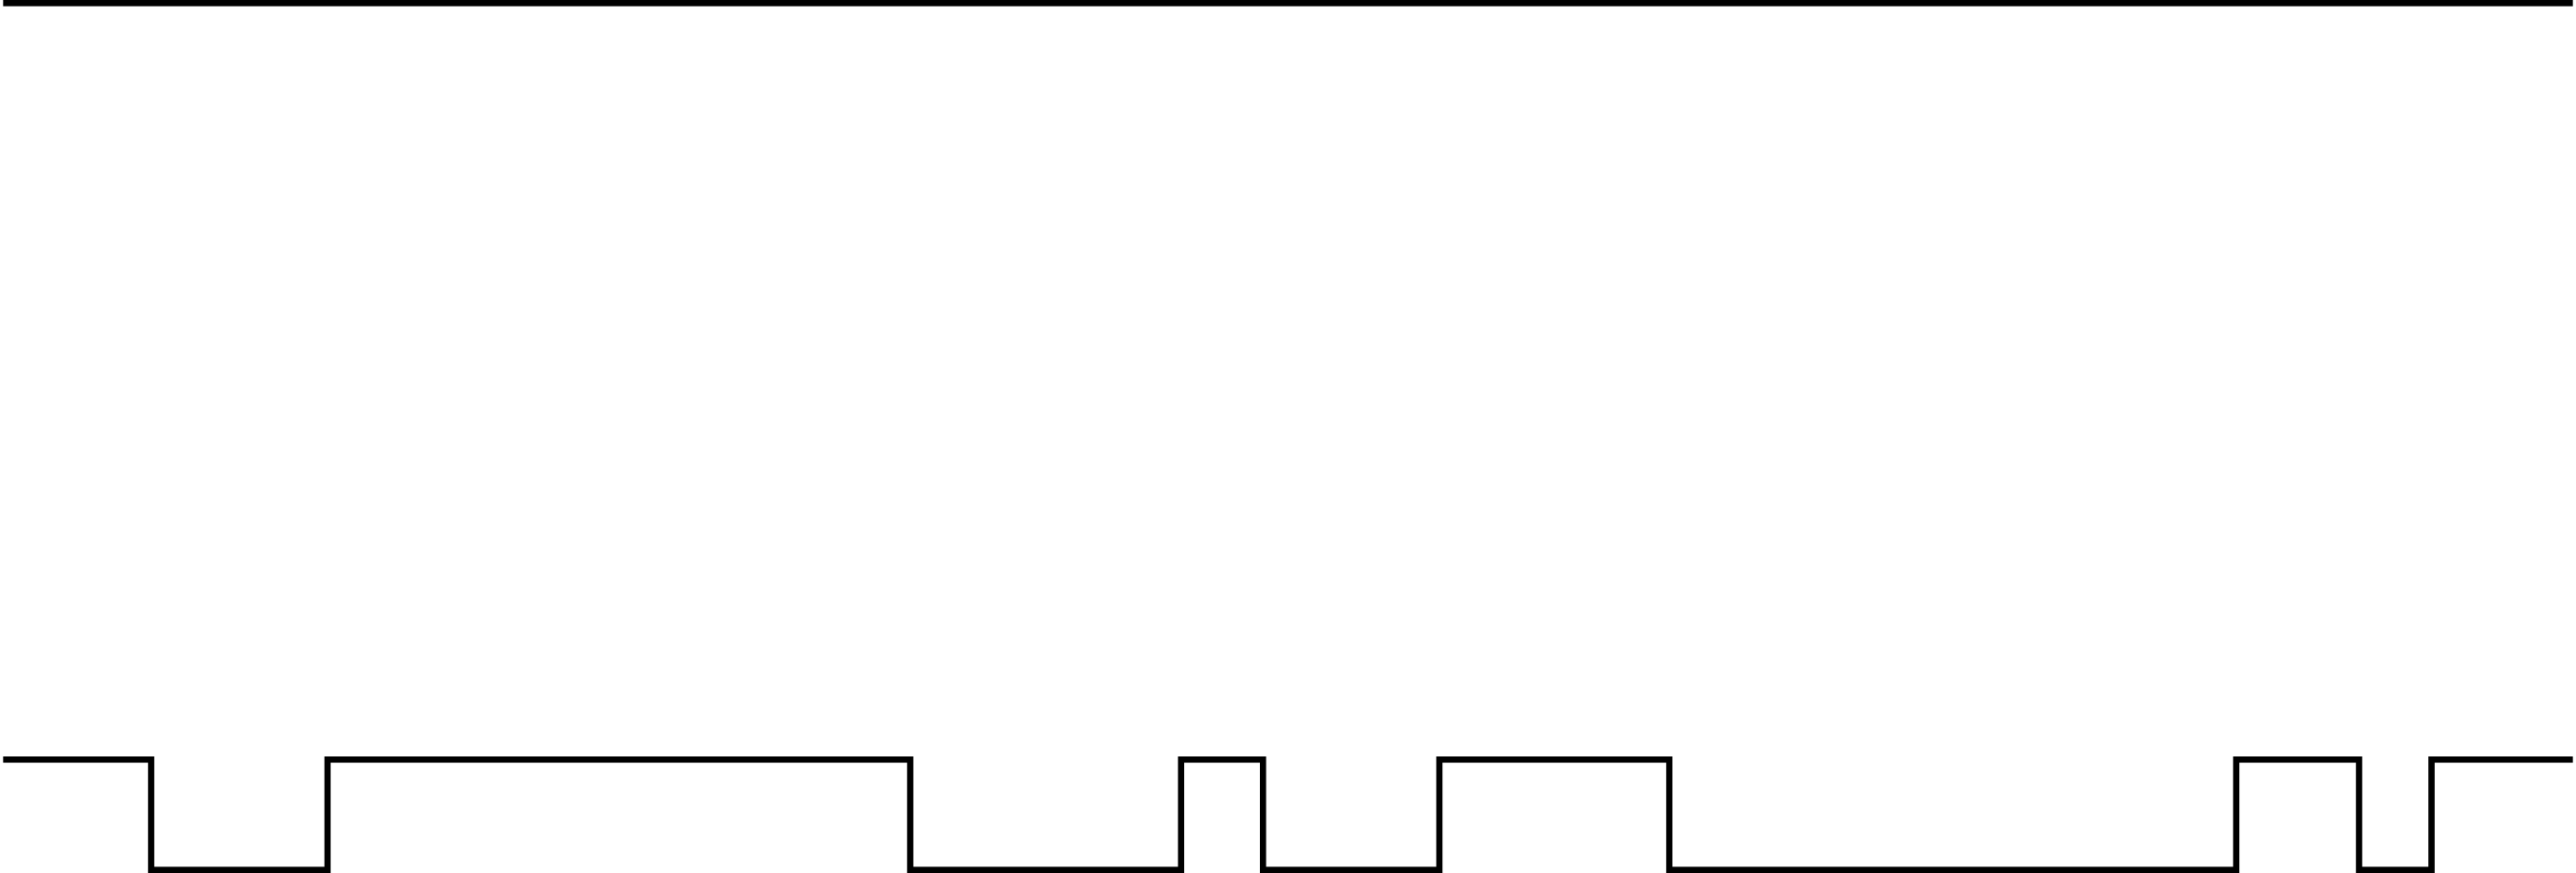
\includegraphics[width=.5\textwidth]{images/topography}
	\caption{Different topographies for the left track and the right track when the ground is smooth on the left side and bumpy on the right side. The top line is for the left track and the bottom line is for the right track.}
	\label{fig:topography}
\end{figure}

\section{The Kalman Filter}
Kalman filters, and even control systems (see Chapter \ref{sec:controls}), use the idea of a state space to encapsulate all of the relevant information that is known about a system such as position, orientation, velocity and acceleration. The standard equations to describe the state space of a system are
\begin{align}
\label{eq:statespace}
\begin{split}
\dot{x} &= f(x,u,t) \\
\dot{y} &= h(x,t)
\end{split}
\end{align}

The ACS Kalman filter is typical of all Kalman filters in that it consists of a prediction update step and a measurement update step where the prediction update is run as fast as possible and the measurement update is run whenever new sensor data becomes available as in Figure \ref{fig:kf}. The prediction update step uses the model of the dynamics of the system and a measurement of elapsed time to determine where the system is in the world. The measurement update step is basically a feedback step to help correct for errors in the system model \cite{Kelly_1994_338}.

\begin{figure}[ht!]
	\centering
	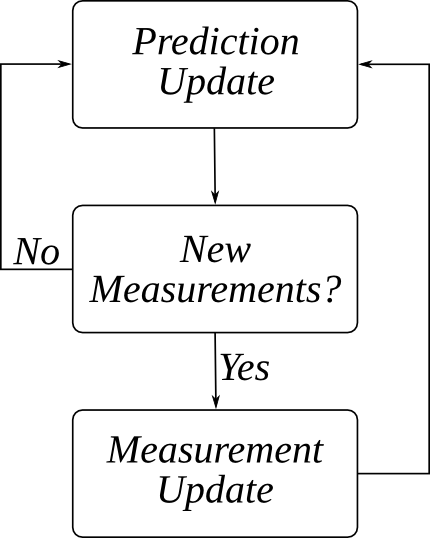
\includegraphics[width=.4\textwidth]{images/kf}
	\caption{The Kalman filter algorithm.}
	\label{fig:kf}
\end{figure}

From \cite{Kelly_1994_338}, \cite{Simon06OptimalEstimation} the prediction update step marches the system dynamics forward in time using the equations
\begin{align}
\label{eq:predictionupdate}
\begin{split}
\hat{x}_{k+1}^- &= \Phi_k\hat{x}_k \\
P_{k+1}^- &= \Phi_kP_k\Phi_k^T + \Gamma_kQ_k\Gamma_k^T
\end{split}
\end{align}
and the measurement update step provides feedback from sensor data using the equations
\begin{align}
\label{eq:measurementupdate}
\begin{split}
K_k &= P_k^-H_k^T\left[H_kP_k^-H_k^T + R_k\right]^{-1} \\
\hat{x}_k &= \hat{x}_k^- + K_k\left[z_k - H_k\hat{x}_k^-\right] \\
P_k &= \left[I - K_kH_k\right]P_k^-
\end{split}
\end{align}

The state space equations for the robot are
\begin{align}
\label{eq:discretess}
\begin{split}
x_{k+1} &= \Phi_kx_k + \Gamma_kw_k \\
z_k &= H_kx_k + v_k
\end{split}
\end{align}

\section{Adaptive Extended Kalman Filter}
*** I really need to clean up the language here. \cite{Busse03adaptiveEKF} looks like a great source. Even the notation as far as \textit{a priori} and \textit{a posteriori} needs fixing. *** Attempting to determine the proper values for the covariance matrices $Q$ in (\ref{eq:predictionupdate}) and $R$ in (\ref{eq:measurementupdate}) can be a laborious process and is often considered more of an art than a science with engineer experience being a critical factor. *** Discuss why $Q$ and $R$ are important and what function they serve in the Kalman filter. *** The ACS Kalman filter has been implemented with an adaptive scheme to update the covariance matrices in real time as the robot moves around and sensor measurements are taken into account \cite{Sights06}, \cite{Mehra72}, \cite{Busse03adaptiveEKF}. $Q$ and $R$ are updated at alternating time steps in the EKF.

The first step is to calculate $Q^\ast$ using
\begin{align}
\label{eq:qstar}
Q^\ast = \left(x-x_{k+1}^-\right)\left(x-x_{k+1}^-\right)^T + P_{k+1}^- - P - Q
\end{align}
Then $Q$ can be updated using
\begin{align}
\label{eq:q}
Q = Q + \frac{1}{L_Q}\left(Q^\ast-Q\right)
\end{align}

Next $R^\ast$ is calculated using
\begin{align}
\label{eq:rstar}
R^\ast = \left(y-Hx\right)\left(y-Hx\right)^T - HP_{k+1}^-H^T
\end{align}
and $R$ can be updated using
\begin{align}
\label{eq:r}
R = R + \frac{1}{L_R}\left(R^\ast-R\right)
\end{align}

*** Discuss the implications of the adaptive EKF. ***

\section{Discriminative Training of Kalman Filter Parameters}
*** Investigate the difference between adaptive filtering and training. It seems like they accomplish the same thing, namely, convergence to some values for the covariance matrices. Do they use the same metrics? Do they converge to the same covariance matrices? Is it just online vs. offline training? *** \cite{Abbeel-RSS-05} describes a method to automatically learn what the covariance matrices should be. When used in conjunction with the adaptive EKF scheme this could allow for faster convergence times when the robots are started and for smaller ranges for the adaptation coefficients $L_Q$ and $L_R$ in (\ref{eq:q}) and (\ref{eq:r}).

\section{Identifty IMU Parameters}
\chapter{Controls}
\label{ch:controls}
Control systems are responsible for computing the commands necessary for actuators to cause the trajectory of a system to go from its current state to a desired state. There are many different methods that can be used to determine the output commands. One of the more popular and widely implemented control systems is the PID (Proportional, Integral, Differential) controller. Lyapunov controllers utilize knowledge of the system dynamics to compute appropriate output commands. The robots in these experiments originally used PID controllers for position and heading control and were later tested with a Lyapunov contoller.

\section{PID}
\label{sec:pid}
PID controllers use the current state estimate to determine the errors between the desired state and the current state. The goal of the PID controller is to drive those errors to zero based on a number of criterion including rise time, settling time, steady state error and overshoot (see Figure \ref{fig:pid}).

\begin{figure}[ht!]
	\centering
	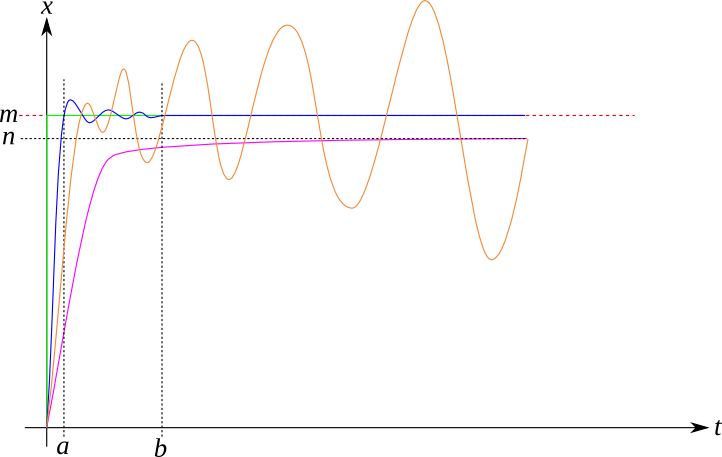
\includegraphics[width=.75\textwidth]{images/pid}
	\caption{PID controller output. The green line is the ideal output while the blue and purple lines are typical results. The orange line shows what happens when a system becomes unstable. Point $m$ represents the desired state, $m-n$ represents steady state error, point $a$ is the rise time and point $b$ is the settling time.}
	\label{fig:pid}
\end{figure}

There are separate PID controllers used for each of $x$ position, $y$ position and robot heading ($\psi$). The process used to compute an output using a PID controller uses three separate errors and a gain for each of those errors. Looking at the PID controller for heading the errors are

\begin{align}
\label{eq:piderrors}
\begin{split}
E_P &= \psi_{\text{ref}_k} - \psi_k \\
E_I &= \sum_{i=0}^{k}E_{P_i}*\Delta T \\
E_D &= \frac{\psi_k - \psi_{k-1}}{\Delta T}
\end{split}
\end{align}
where $\psi_{\text{ref}_k}$ is the desired heading at the current time, $\psi_k$ is the current heading estimate, $\psi_{k-1}$ is the previous heading estimate and $\Delta T$ is the time elapsed since the last PID control calculation was performed. The contribution of each error is then weighted by a gain to obtain the final output command, $u$, such that

\begin{align}
\label{eq:pidcommand}
u = K_P*E_P + K_I*E_I + K_D*E_D
\end{align}
where $K_P$ is the proportional gain, $K_I$ is the integral gain and $K_D$ is the differential gain.

The only parameters available to tune PID controllers for performance are the gains. There are some rules of thumb for tuning gains properly as described in \cite{ZeiglerNichols42} that can work as a good starting point. The difficulty in using PID controllers for the small robots used in these experiments is that the gains must be tuned for specific operating scenarios so that a set of gains that work well at full speed on asphalt do not work at all when the robot is driving in soft sand at any velocity. PID controllers work best when they only have to reject a small range of disturbances and the small robots are required to be operated in environments with a large range of disturbances.

When the characteristics of a robot are changed the PID gains must also be modified to reflect those changes. These characteristics include mass, center of mass, particular treads or motors and payloads, as these all affect the dynamics of the system. Gain scheduling is the process of tuning a system to use a different set of gains based on the operating environment or characteristics of the robot, however this is very time consuming. This motivates the search for a better control system for these small robots.

\section{Lyapunov}
\label{sec:lyapunov}
*** Talk about how Lyapunov controllers work \cite{Khalil02}. Show which control Lyapunov function I chose \cite{Rusu05RobotuxLyapunov}. For a given path show the linear and angular velocities that are output by each controller. ***
\chapter{Results}
\label{ch:results}
*** I want to show plots with the position estimate using GPS only, KF with learned Q/R but no adapting, KF with no adapting or training, KF with adapting, KF with learned and adaptive, KF with different encoder equations. Would be cool to plot these on an overhead image of the test area. ***

*** I want to show plots of the variance of the KF position estimate and the derivative of the control outputs of linear and angular velocity. The real goal is to have smooth velocities which will show up as constant accelerations and I want to see if there is any correlation between the variance of the position estimate and the accelerations, especially when the variance of the position esimate has a large amplitude. This would indicate that the controller is not necessarily doing a poor job and I could relate this to the example of the robot controller causing the robot to spin in circles when the IMU is giving faulty outputs. Note that this would not be a sufficient condition to show that the controller is performing properly but would only be an indication that the KF output needs improvement. There are likely ways of assessing controller performance if the KF output variance is large though. ***

\section{Kalman Filter Results}
\label{sec:kfResults}
Using logged data from the Kalman filter running with default $Q$ and $R$ parameters the robot track is shown in Figure \ref{fig:kfPlainDataFirstAttempt}.

\begin{figure}[ht!]
	\centering
	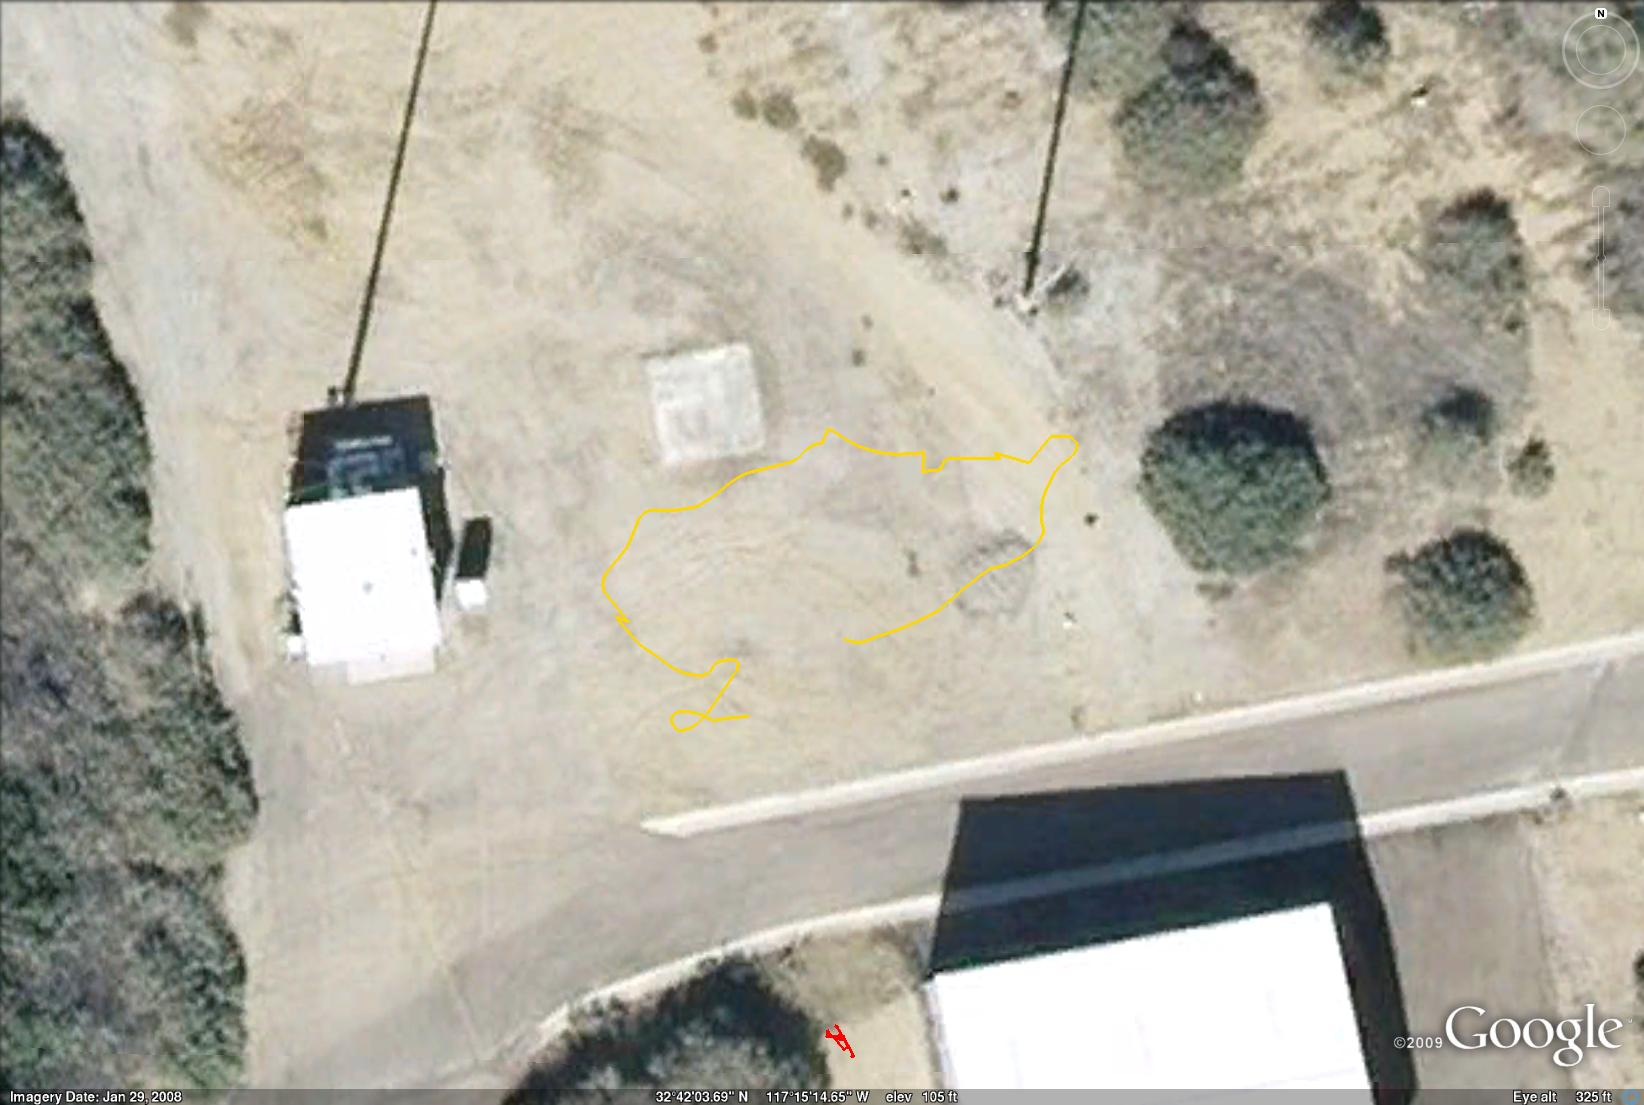
\includegraphics[width=.95\textwidth]{images/kfPlainDataFirstAttempt}
	\caption{Kalman filter output using the default parameters. The robot track is shown in yellow and a static GPS receiver with DGPS corrections is shown in red.}
	\label{fig:kfPlainDataFirstAttempt}
\end{figure}

\section{Lyapunov Controller Results}
\label{sec:lyapunovResults}
The initial attempt at running the Lyapunov controller on the PackBot resulted in rather poor performance that was likely caused by either mismatched units or the wrong equations being used in the code (see Figure \ref{fig:lyapunovDataFirstAttempt}).

\begin{figure}[ht!]
	\centering
	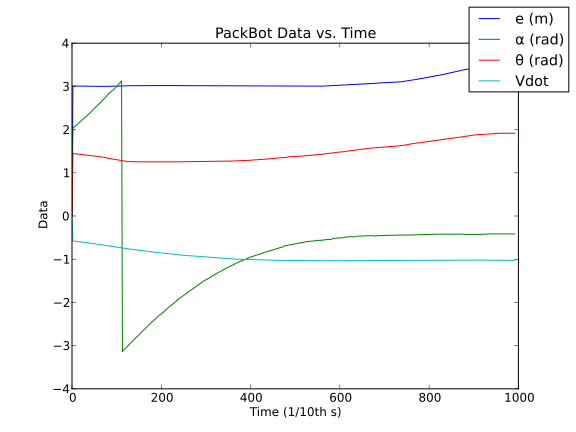
\includegraphics[width=.95\textwidth]{images/pbData}
	\caption{First attempt at running the PackBot using the Lyapunov controller.}
	\label{fig:lyapunovDataFirstAttempt}
\end{figure}
\chapter{Future Work}
\label{ch:futurework}
\begin{enumerate}
\item Use the learning algorithm for indoor robots as there is no reason why a robot needs to have GPS to benefit from using the DGPS system for training the $Q$ and $R$ matrices in the EKF. A test area would need to be set up outdoors so that DGPS can be used and the normal sensors also work by bouncing off walls and what not but the DGPS ground truth position can be converted to the local coordinate system and used to generate an error metric for the EKF position output.
\item Add a high quality IMU that serves as ground truth for Euler angles to the DGPS system so that the training algorithm attempts to minimize the errors between Euler angles in addition to position.
\item Develop a better method for training the EKF covariance matrices by using a better parameter search algorithm or by massively parallelizing the current naive, brute force algorithm. Since determining all of the possible matrices is relatively inexpensive compared to simulating the EKF output all of the possible matrices for a particular grid size can be generated and stored in memory and then the EKF can be run simultaneously using each of those matrices where the next grid step uses the $Q$ and $R$ that minimized the output error of the EKF.
\item Characterize individual IMUs better since that is a large source of error.
\item Instead of the naive, brute force method of trying all the $Q$ and $R$ matrices use a better machine learning algorithm. This could either be a neural network using FANN or a gradient descent approach that leads the elements of $Q$ and $R$ in the proper direction when minimizing the derivative of the errors computed using either the residual or the prediction error metrics. It would be great to try all of the different methods, have theory showing which ones should work better and then have data to show how well the results match with the theory. Some analysis of which methods work best and under what circumstances would be hugely beneficial, not to mention interesting.
\end{enumerate}

\chapter{Conclusion}
*** Summarize the results here. ***

\appendix
\chapter{Source Code}
\label{ch:code}
This is some of the source code used in this research. Contact the \mailto{\thesisAuthorEmail}{author} for more complete listings.

\section{QR}
\label{sec:qrcode}
This code was used to generate the $Q$ and $R$ matrices.
% Set the syntax highlighting to C++.
\lstset{language=C++}
\matlabscript{code/qr/qr.cc}{Main C++ file for genearating $Q$ and $R$ matrices.}

\clearpage
\section{DGPS}
\label{sec:dgpscode}
This code was used to set up and communicate with DGPS receivers.
\matlabscript{code/gpslogger/gpslogger.cpp}{Main C/C++ file for logging GPS data.}
% \matlabscript{code/gpslogger/oem4.cpp}{Main C++ file for the Novatel OEM4 library.}

\clearpage
\section{Lyapunov}
\label{sec:lyapunovcode}
This code was adapted from \cite{Rusu05RobotuxLyapunov}. Most of the changes involved making the code more efficient and adding additional comments.
% Set the syntax highlighting back to Matlab.
\lstset{language=Matlab}
\matlabscript{code/lyapunovRusu/main.m}{Main Matlab file for Lyapunov controller.}
\matlabscript{code/lyapunovRusu/f3.m}{Matlab file for ODE solver for Lyapunov controller.}
\matlabscript{code/lyapunovRusu/CalcETA.m}{Matlab file for calculating the robot trajectory for Lyapunov controller.}


% Bibliography.
\bibliographystyle{these}
\bibliography{mybib}

\end{document}